\begin{frame}
    \centering
    \begin{figure}[H]
        
\includegraphics[keepaspectratio, width=0.7\paperwidth, height=\paperheight]{Logos/FreeFlower.pdf}
    \end{figure}
    Elternabend der Klasse 1c,\\
    05. September 2024
\end{frame}

\begin{frame}[fragile]{Ablauf des Elternabends}
\begin{itemize}[<+->]
    \item Teil 1: Musiksaal 18:30 - 19:30 \emoji{check-mark}\\ 
      Begrüssung und Informationen durch Arno Germann (Rektor) und Stephan Schönenberger (Prorektor und Jahrgangsbetreuer)    
	  \item Teil 2: Zimmer 504, 19:15 bis $\approx$ 20:00
      \begin{itemize}
        \item Fachlehrpersonen und Klassenlehrer stellen sich vor
        \item Kurzporträts der Schülerinnen und Schüler
        \item Klassentag und Klassenlager
        \item Schulleitung und Klassenlehrperson
        \item Fragen (im Plenum)
      \end{itemize}
    \item Teil 3: ungezwungener Austausch beim Apéro \emoji{cocktail-glass}
    \end{itemize}
\end{frame}

\begin{frame}
\centering
  \begin{figure}[H]
      
\includegraphics[keepaspectratio, width=0.7\paperwidth, height=\paperheight]{Logos/FreeFlower.pdf}
  \end{figure}
  Fachlehrpersonen und Klassenlehrer stellen sich vor
\end{frame}

\begin{frame}[fragile]{Fächer und Lehrpersonen}
  \centering
  \begin{table}[H]
  \adjustbox{max width=\textwidth}{%
  \begin{tabular}{l
  >{\columncolor[HTML]{FFFFFF}}l |ll}
  \textbf{Lehrperson}    & \textbf{Fach} & \textbf{Lehrperson} & \textbf{Lehrperson}        \\ \hline
  Wolfgang Pils          & Physik        & Selina Frölicher    & Bildnerisches Gestalten    \\ \hline
  Frigge Lengerer        & Englisch      & Stefanie Bäurle\footnote{{\tiny heute an Sitzung der Prüfungskommission der zentralen Aufnahme Prüfung}}     & Deutsch                    \\ \hline
  Peter Nussbaumer       & Musik         & Thomas Graf         & Klassenstunde / Informatik \\ \hline
  Katia Bescotti         & Italienisch   & Milos Stolic        & Bildnerisches Gestalten    \\ \hline
  Corinne Hübscher       & Französisch   & Christoph Itzel     & Sport                      \\ \hline
  Daniel Merki           & Chemie        & Simon Gallmann      & Sport                      \\ \hline
  Thomas Foertsch        & Mathematik    & Aline Schneider     & Biologie                   \\ \hline
  Olivia Batchelor-Travé & Geschichte    & Mirja Zuber         & Mathematik                 \\ \hline
    \end{tabular}}
  \end{table}
\end{frame}

\begin{frame}[fragile]{zu meiner Person}
  \begin{itemize}[<+->]
    \item Informatiklehrer an der KS Im Lee
    \item wohne in Effretikon mit meiner Verlobten und zwei Katzen
  \end{itemize}
\end{frame}

\begin{frame}
\centering
  \begin{figure}[H]
      
\includegraphics[keepaspectratio, width=0.7\paperwidth, height=\paperheight]{Logos/FreeFlower.pdf}
  \end{figure}
  Kurzporträts der Schülerinnen und Schüler 
\end{frame}

\begin{frame}
\centering
  \begin{figure}[H]
      
\includegraphics[keepaspectratio, width=0.7\paperwidth, height=\paperheight]{Logos/FreeFlower.pdf}
  \end{figure}
  Klassentag und Klassenlager
\end{frame}

\begin{frame}[fragile]{Klassentag (Teil 1 von 2)}
\begin{itemize}
  \item Am Dienstag, 10. September 2024 wird der Klassentag der Klasse 1c stattfinden (wirklich? \emoji{cloud-with-rain}\emoji{cloud-with-lightning}). Das Verschiebedatum bei schlechtem Wetter ist der Freitag, 13. September 2024. 
  \item Ziel des Klassentags ist die gemeinsame Planung des Klassenlagers. Die Schülerinnen und Schüler werden Menüpläne und Einkaufslisten ausarbeiten und Abendunterhaltungen konzipieren. 
  \item Zudem bietet der Klassentag eine gute Gelegenheit, sich untereinander besser kennenzulernen und auszutauschen.
\end{itemize}
\end{frame}

\begin{frame}[fragile]{Klassentag (Teil 2 von 2)}
Am Mittag werden wir zusammen in den Wald oben beim Goldenberg gehen, ein Feuer anzünden und ein individuell mitgebrachtes Mittagessen einnehmen (Würste, Sandwiches, anderes Grillgut, $\ldots$).
\begin{description}
  \item[Grillstelle 1. Wahl:] \url{https://maps.app.goo.gl/3p5Uh1vmMrhA3anR9}
  \item[Grillstelle 2. Wahl:] \url{https://maps.app.goo.gl/dsiK2Exe1Hv661Eb6}
\end{description}
Abgesehen von dem Mittagessen wird der Klassentag im Schulhaus stattfinden.
\end{frame}


\begin{frame}[fragile]{Klassenlager (Eckdaten)}
\begin{itemize}[<+->]
  \item Das Klassenlager wird am Montag, 30. September 2024 beginnen (Abfahrt ab Winterthur HB: 07:09 Uhr) und am Freitag, 04. Oktober 2024 enden (Ankunft im Winterthur HB: 16:51 Uhr).
  \item Unsere Unterkunft wird das \textit{Ferienhaus Madulain} im Engadin sein: \url{https://www.ferienhaus-madulain.ch/unterkunft}.
  \item Ferienhaus Madulain auf Google Maps: \url{https://tinyurl.com/FerienhausMadulain}
  \item Leitung: Stefanie Bäurle (Deutschlehrerin der Klasse 1c), Thomas Graf
\end{itemize}
\end{frame}

\begin{frame}[fragile]{Klassenlager (Wochenplan)}
\centering
\begin{table}[]
\begin{adjustbox}{center}
\resizebox{1.15\textwidth}{!}{%
\begin{tabular}{|l|l|l|l|l|}
\hline
\textbf{Mo, 30.09.2024} &
  \textbf{Di, 01.10.2024} &
  \textbf{Mi, 02.10.2024} &
  \textbf{Do, 03.10.2024} &
  \textbf{Fr, 04.10.2024} \\ \hline
\begin{tabular}[c]{@{}l@{}}Abfahrt: 07:09, Ankunft: 10:29\\ gemeinsames Mittagessen\end{tabular} &
  Frühstück &
  Frühstück &
  Frühstück &
  Frühstück \\ \hline
\begin{tabular}[c]{@{}l@{}}Ortschaft erkunden\\ freie Zeit\end{tabular} &
  \begin{tabular}[c]{@{}l@{}}Seen\\ (Silvaplanasee, Sils,\\ St. Moritz, Surlej)\end{tabular} &
  Nationalpark \textit{Val Trupchun} &
  Morteratschgletscher &
  \begin{tabular}[c]{@{}l@{}}Putzen, Packen\\ Wegzehrung vorbereiten\end{tabular} \\ \hline
\begin{tabular}[c]{@{}l@{}}Nachtessen\\ Abendunterhaltung\end{tabular} &
  \begin{tabular}[c]{@{}l@{}}Nachtessen\\ Abendunterhaltung\end{tabular} &
  \begin{tabular}[c]{@{}l@{}}Nachtessen\\ Abendunterhaltung\end{tabular} &
  \begin{tabular}[c]{@{}l@{}}Nachtessen\\ Abendunterhaltung\end{tabular} &
  \begin{tabular}[c]{@{}l@{}}Abfahrt: 13:23, Ankunft: 16:51\\ Ferien \emoji{beach-with-umbrella}\end{tabular} \\ \hline
\end{tabular}%
}
\end{adjustbox}
\end{table}
\end{frame}


\begin{frame}
\centering
  \begin{figure}[H]
      
\includegraphics[keepaspectratio, width=0.7\paperwidth, height=\paperheight]{Logos/FreeFlower.pdf}
  \end{figure}
  Schulleitung und Klassenlehrperson
\end{frame}

\begin{frame}[fragile]{Schulleitung}
  \begin{description}
    \item[Rektor:] Arno Germann
    \item[Prorektorin:] Susanna Schaad
    \item[Prorektor:] \text{Stephan Schönenberger} (Jahrgangsbetreuer)
  \end{description}
\end{frame}

\begin{frame}[fragile]{Klassenlehrperson}
  \begin{description}[<+->]
    \item[Bezugs- und Vertrauensperson:] Anlaufstelle bei schulischen und (teils) ausserschulischen Problemen
    \item[Verantwortung:] Verantwortung für das Zusammenleben, das Arbeitsklima und Disziplin
    \item[Vermittlung:] bei Problemen: Kontaktaufnahme mit den Eltern, Vermittlung mit Fachlehrpersonen
    \item[Organisation:] Klassentag, Klassenlager, administrative Pflichten (e.g. Absenzenwesen)
  \end{description}
\end{frame}


\begin{frame}[fragile]{Rollenverteilung}
  \centering
  \begin{figure}[H]
      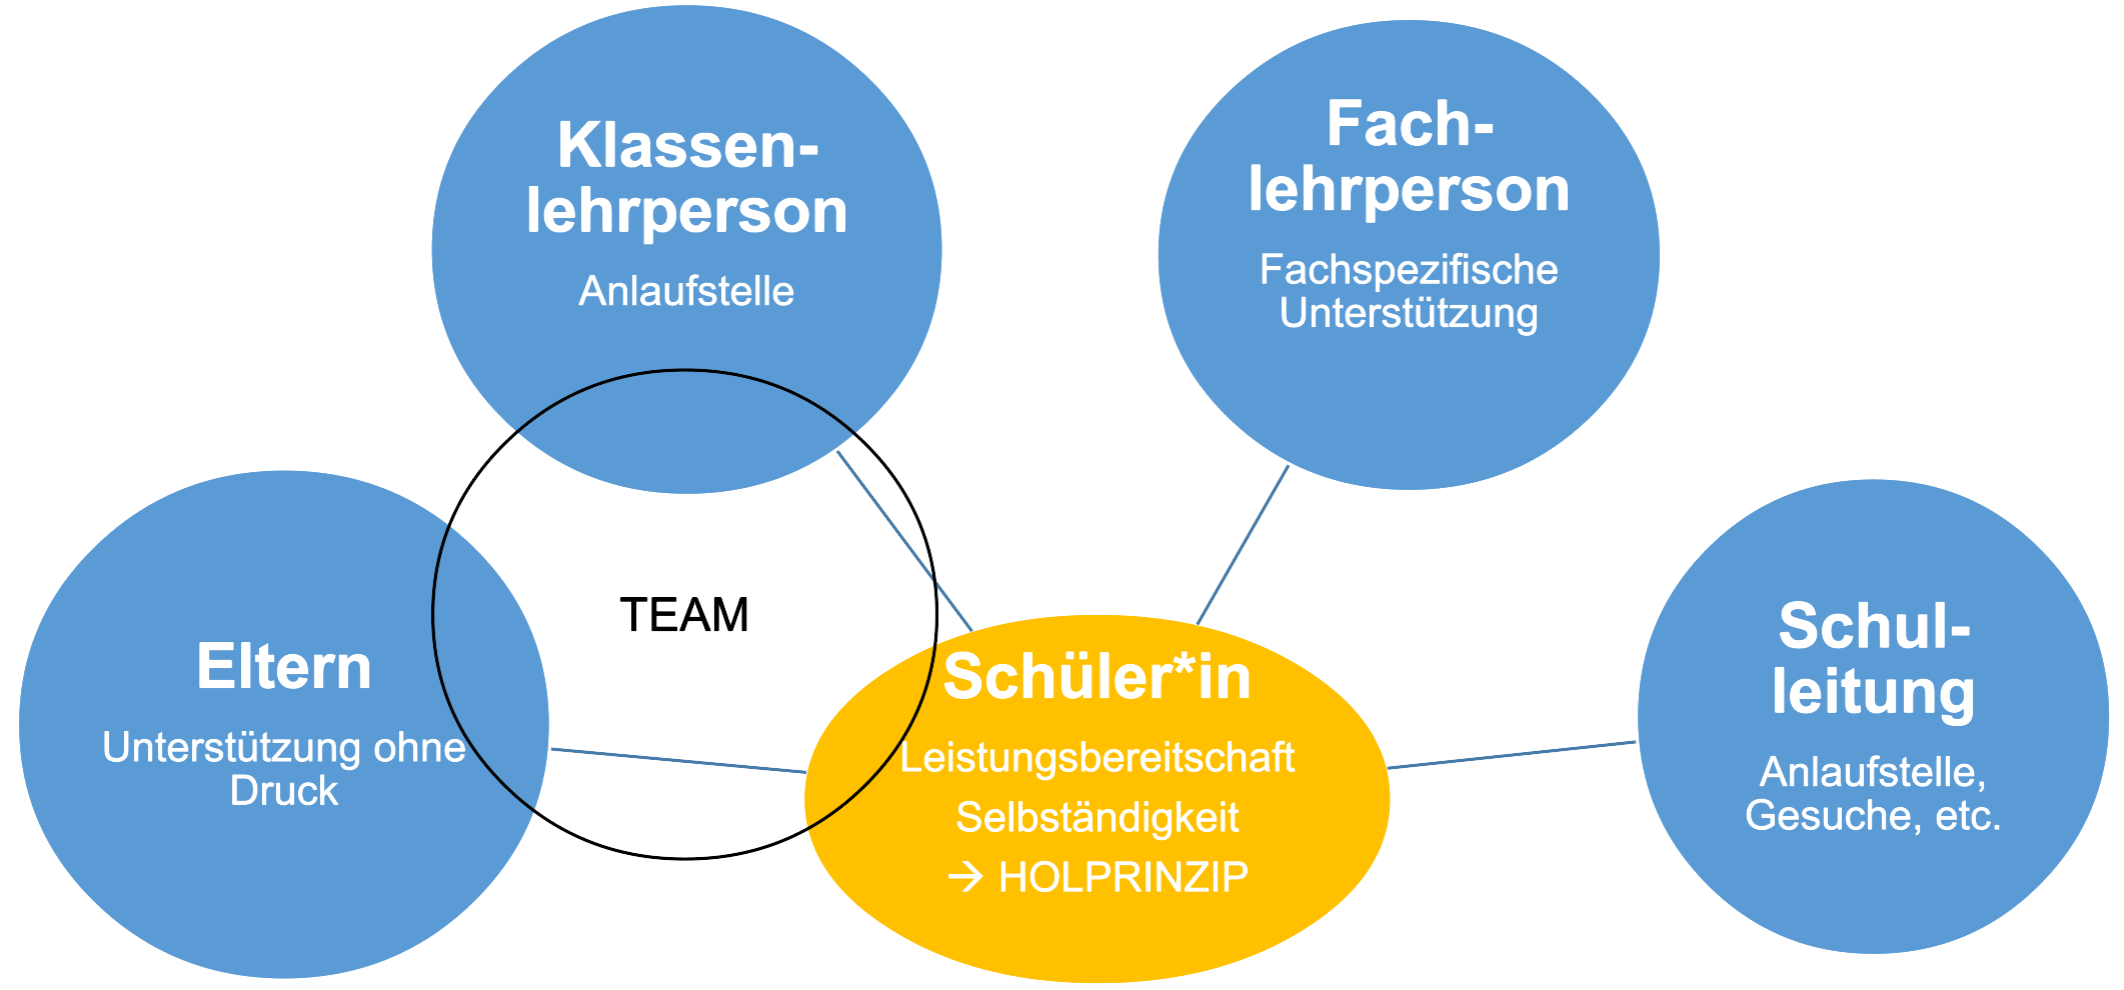
\includegraphics[keepaspectratio, width=0.7\paperwidth, height=\paperheight]{Klassenstunde/Rollen.png}
  \end{figure}
\end{frame}

\begin{frame}[fragile]{Was ist neu an der Kantonsschule?}
  \begin{itemize}[<+->]
    \item \textcolor{Red}{gleichzeitig mehr Fächer} $\rightarrow$ \textcolor{Green}{Material gut organisieren (Laptop, Ordnerstruktur, Dateiablage)}
    \item \textcolor{Red}{höhere Ansprüche (kognitiv, fachlich, Genauigkeit)} $\rightarrow$ \textcolor{Green}{mehr Einsatz, Gelassenheit gegenüber tieferen Noten}
    \item \textcolor{Red}{mehr Lehrperson, Reduktion der persönlichen Bindung und Betreuung} $\rightarrow$ \textcolor{Green}{Flexibilität, Eigenständigkeit}
  \end{itemize}
\end{frame}

\begin{frame}[fragile]{Bewährte Tipps}
  \begin{itemize}[<+->]
    \item keine Lücken entstehen lassen, Kolleginnen und Kollegen Fragen, Eltern beziehen (allenfalls Nachhilfe beanspruchen)
    \item bei Unklarheiten: Fragen stellen, kommunizieren
    \item nach schlechtem Start nicht schon aufgeben
    \item sich auch für ungeliebte Fächer motivieren
    \item ungenügende Noten erhöhen hat mehr Wirkung als genügende Noten weiter zu verbessern (Stichwort: doppelte Kompensation)
    \item zusammen lernen
  \end{itemize}
\end{frame}

\begin{frame}[fragile]{Hilfsangebote}
  \begin{itemize}[<+->]
    \item \url{https://www.ksimlee.ch/}
    \item schulinterne Beratungs- und Anlaufstellen 
    \item Stipendien 
    \item Studien- und Laufbahnberatung
  \end{itemize}
\end{frame}

\begin{frame}{Adressliste überprüfen}
\centering
  \begin{figure}[H]
      
\includegraphics[keepaspectratio, width=0.7\paperwidth, height=\paperheight]{Logos/FreeFlower.pdf}
  \end{figure}
  Bitte überprüfen Sie Ihre Angaben.\\ 
  \emoji{cross-mark}\emoji{camera} keine Fotos \emoji{camera}\emoji{cross-mark}
\end{frame}

\begin{frame}
\centering
  \begin{figure}[H]
      
\includegraphics[keepaspectratio, width=0.7\paperwidth, height=\paperheight]{Logos/FreeFlower.pdf}
  \end{figure}
  Fragen (im Plenum) 
\end{frame}


\begin{frame}
\centering
  \begin{figure}[H]
      
\includegraphics[keepaspectratio, width=0.7\paperwidth, height=\paperheight]{Logos/FreeFlower.pdf}
  \end{figure}
  \emoji{tropical-drink} Vielen Dank für Ihre Zeit! \emoji{clinking-glasses} 
\end{frame}
